\section{Evaluation}
\label{sec:eval}

\begin{figure}[!ht]
\begin{center}
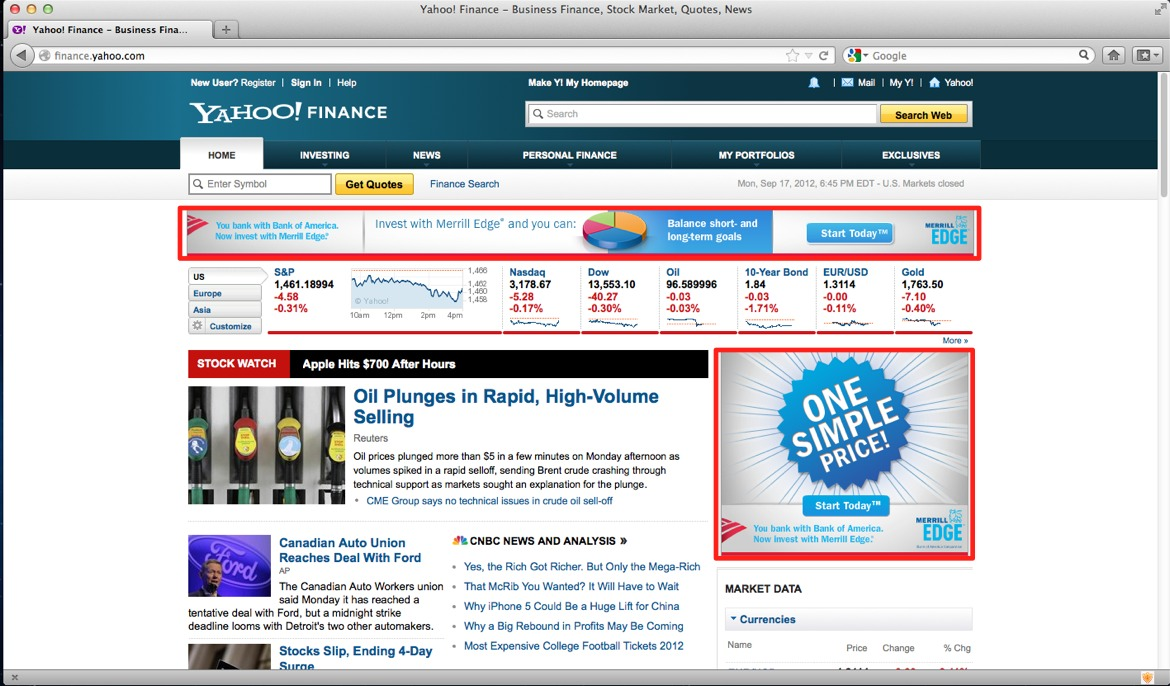
\includegraphics[width=0.7\textwidth]{before-csp23}
\end{center}
\caption{Before any Content Security Policy is applied to {\it http://finance.yahoo.com/} web site}
\label{fig:beforeCSP}
\end{figure}

We implemented our approach in Firefox v14.0 using JetPack SDK
v1.9. We used Alexa Top 10 Sites \footnote[2]{Alexa top 10 sites used
  for evaluation were: facebook.com, google.co.in, youtube.com,
  yahoo.com, baidu.com, wikipedia.org, live.com, twitter.com, qq.com,
  and amazon.com} to test our approach against user defined CSP
policies as well as automatically inferred CSP policies. Automatically
inferred CSP policies don't break websites whereas manually defined
CSP policies required several rounds of refinement and web page source
code inspection to record content sources. The reason for that is
initially we set CSP rules for a website to load resources from its
own domain only, but websites were loading content from CDN's or
sub-domains. Appendix~\ref{appendix} shows examples of inferred CSP
policies.

\subsection{Effectiveness of Automatically Infer CSP}
We tested effectiveness of UserCSP with Alexa TOP 10 Sites listed in
Appendix ~\ref{appendix}.


\begin{figure}[!ht]
\begin{center}
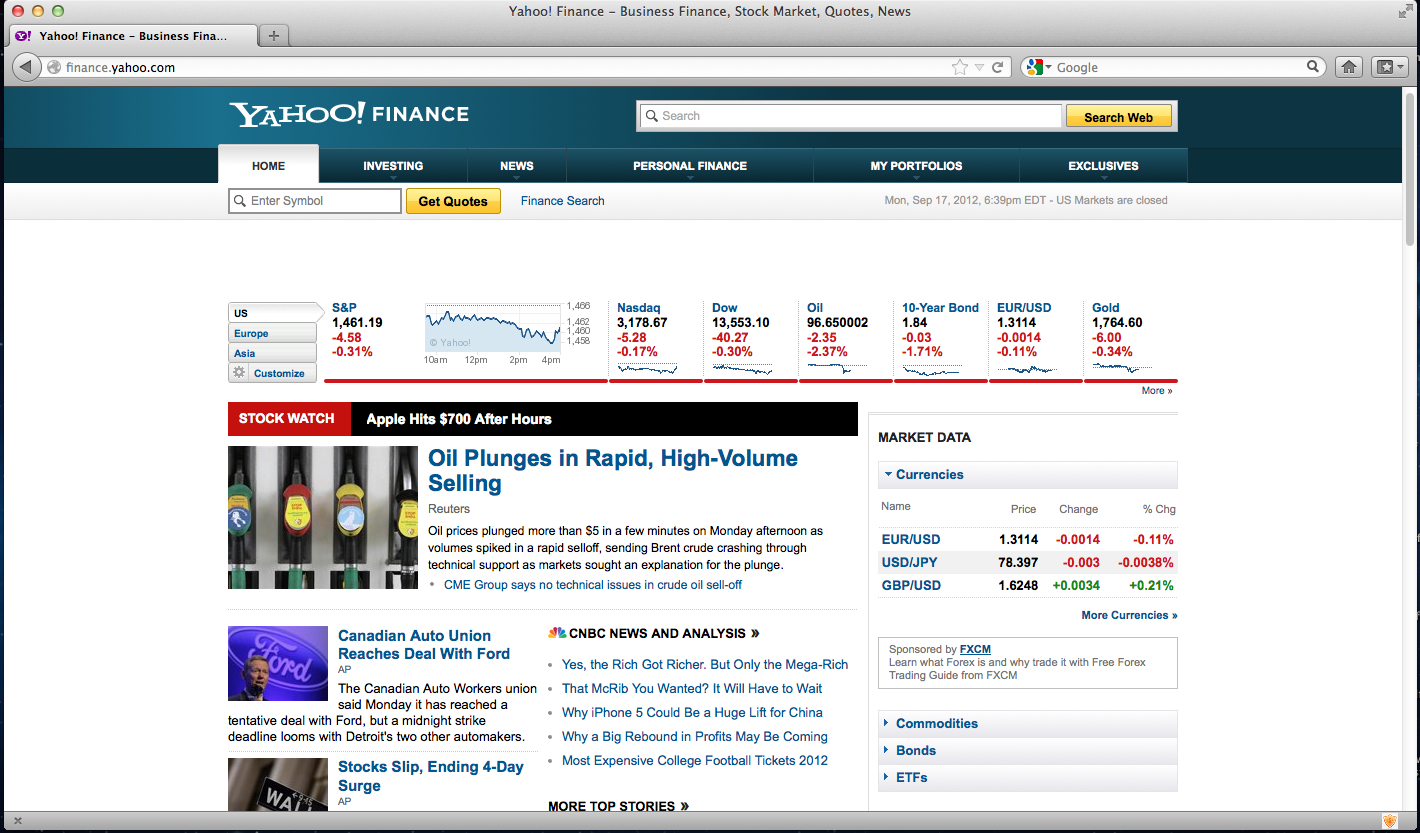
\includegraphics[width=0.7\textwidth]{after-csp23}
\end{center}
\caption{After {\tt object-src:'self'} Content Security Policy is
  applied to {\it http://finance.yahoo.com/} web site}
\label{fig:afterCSP}
\end{figure}

Automatically infer CSP policy feature of UserCSP helps a developer to
derive a usable and secure policy for their web site. By looking at
the content the website loads, the add-on determines the strictest set
of CSP rules it can apply to the site without breaking the current
page. Web users can also protect themselves by disabling content such
as objects on personal finance sites or frames and third party
JavaScript for their web-email.  Figure~\ref{fig:beforeCSP} shows an
example of \url{http://finance.yahoo.com/} web site, which used
third-party flash objects. In the Figure, third-party flash objects
are marked with red rectangle. Figure~\ref{fig:afterCSP} shows an
example, where user specified Content Security Policy that sets {\tt
  object-src} directive to {\tt 'self'} so that third-party plugins
won't load.  All third-party flash object used for an advertisement in
\url{http://finance.yahoo.com/} were blocked by our UserCSP add-on
after the user applied a custom policy.

